\chapter[Sistema Adaptativo de Vídeos Interativos]{Sistema Adaptativo de Vídeos Interativos}

Tendo como base as teorias apresentadas, foi desenvolvido um sistema que utiliza o modelo arquitetural MVC e que contempla duas funcionalidades principais: um módulo para autoria de cursos compostos por vídeos interativos e um módulo para visualização adaptativa destes cursos, que contemple adaptações de conteúdo e navegação. 

Para facilitar a compreensão do trabalho técnico desenvolvido, este capítulo foi subdividido em seis tópicos: modelagem do domínio, suporte tecnológico, arquitetura do software, testes, gerência de configuração e aspectos gerais.

\section{Modelagem do Domínio}

O modelo do domínio do software pretende apresentar os elementos que compõem a lógica do sistema e como eles foram organizados para que os objetivos do trabalho pudessem ser alcançados. É importante ressaltar que estes modelos apresentados foram evoluídos no decorrer do desenvolvimento até alcançarem um nível estável, já que o método seguido foi interativo e incremental segundo as práticas do \textit{Scrum}.

\begin{figure}[h!]
	\centering
  	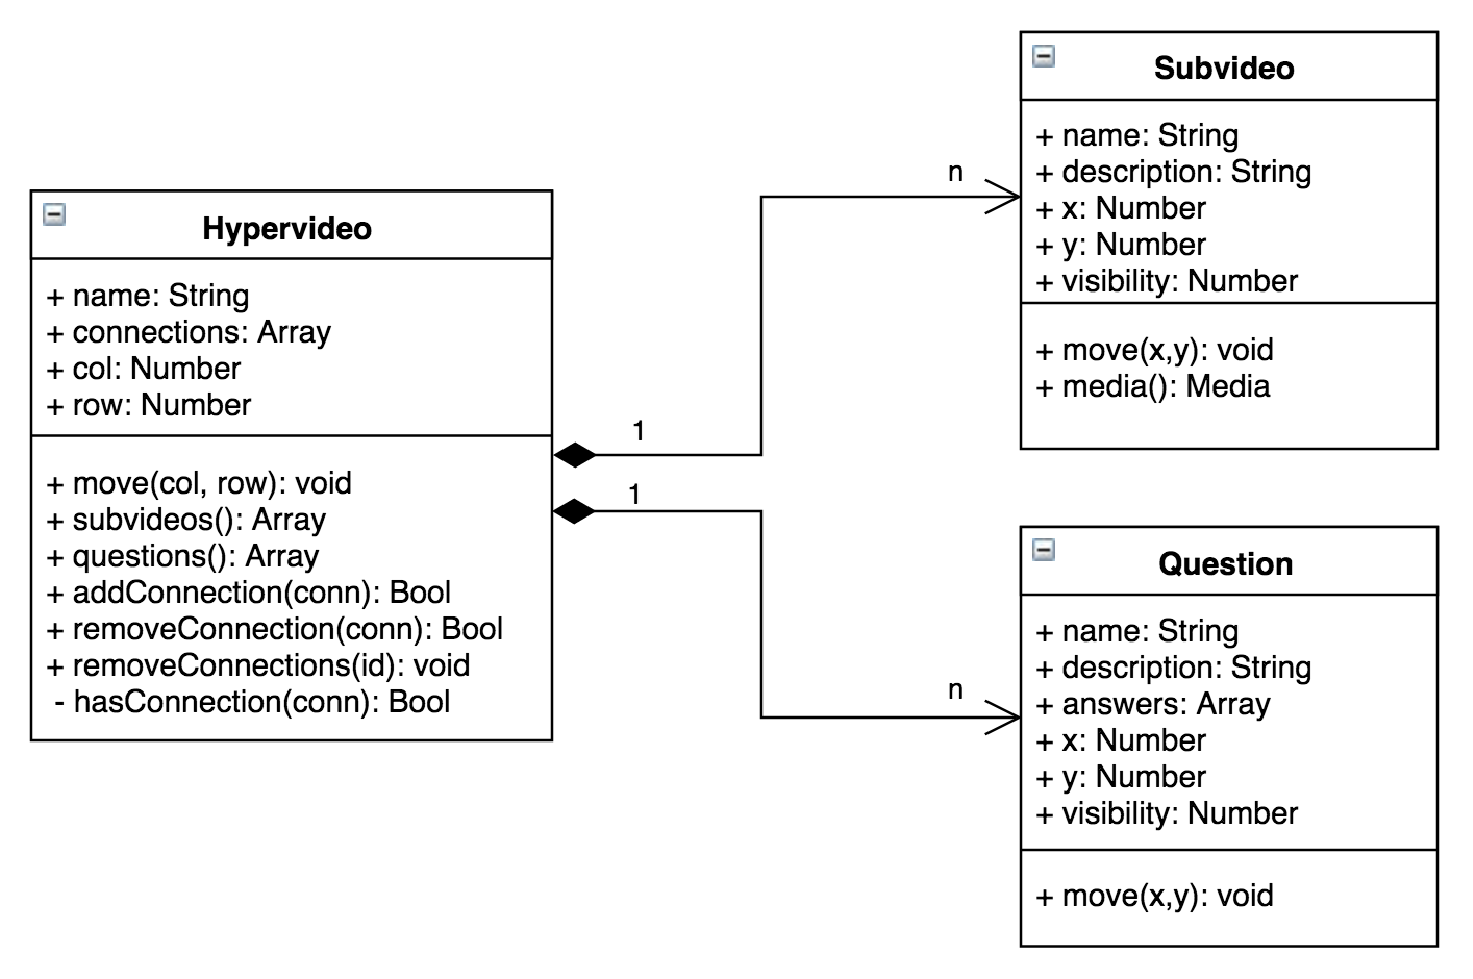
\includegraphics[width=.6\linewidth]{figuras/video.eps}
  	\caption{Diagrama do vídeo interativo proposto}
  	\label{fig:video}
\end{figure}

Primeiramente, foi modelado um vídeo interativo que pudesse ser utilizado na construção de um curso. Levando em consideração os princípios do design multimídia, os vídeos interativos possuem pouco espaço para textos escritos na tela; são formados por subvídeos interligados segundo definido pelo professor autor; possuem questões a serem respondidas ao longo da apresentação do vídeo e devem ser adaptativos segundo os diferentes perfis de usuário. Além disso, um vídeo interativo deve possuir as informações necessárias para que ocorra a quantização da rede, ou seja, para cada usuário que o acesse, deve existir uma avaliação e uma confiabilidade atribuidos a ele, bem como uma posição em um plano bidimensional referente ao mapa conceitual do curso ao qual o vídeo interativo pertence. 

\begin{figure}[h!]
	\centering
  	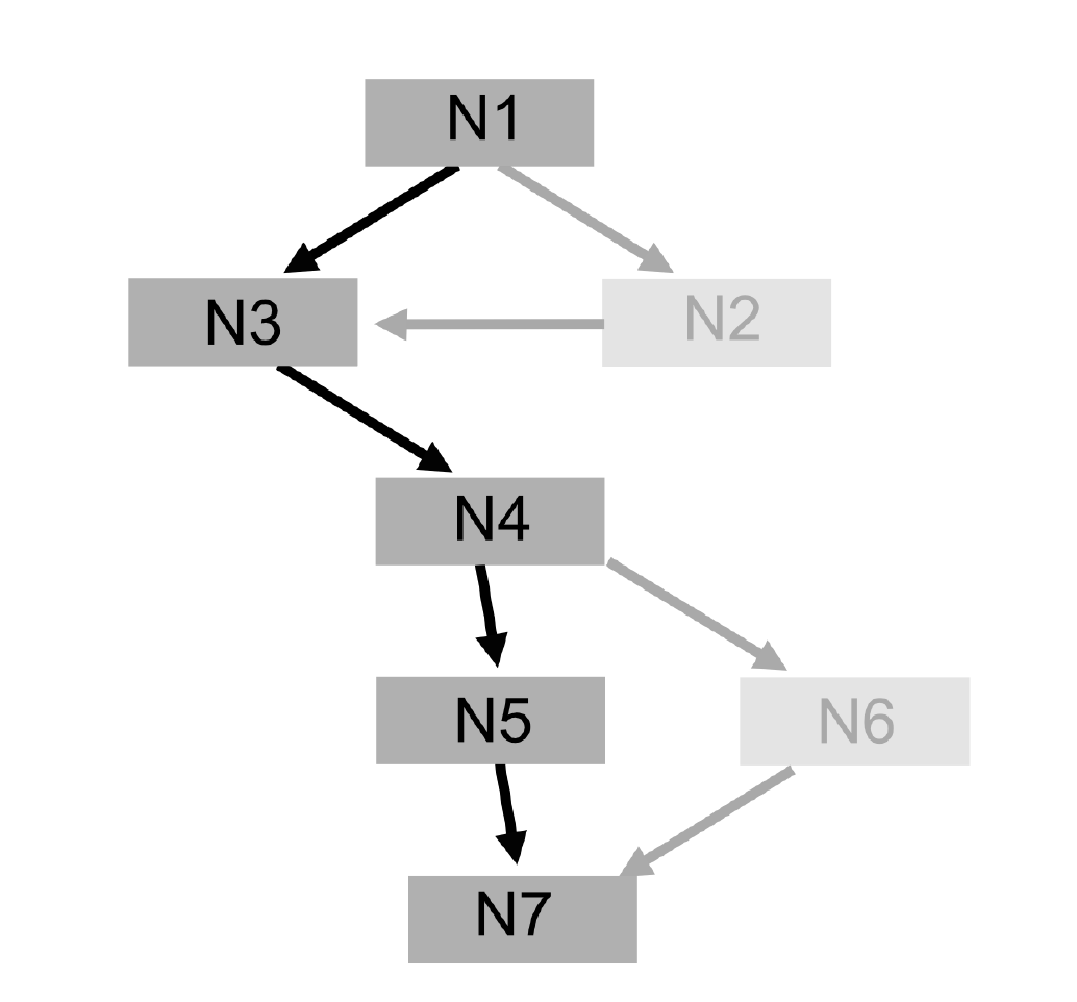
\includegraphics[width=.3\linewidth]{figuras/estrutura.eps}
  	\caption{Adaptação do hypervideo por meio da ocultação dos nodos N2 e N6}
  	\label{fig:estrutura}
\end{figure}

Cada subvídeo possui informações básicas sobre a mídia de vídeo que será apresentada por ele, como título e uma breve descrição do conteúdo. Além disso, possuem um nível de visibilidade para serem apresentados apenas ao perfil específico para o qual foi projetado, garantindo assim a capacidade de adaptação a nível de conteúdo. A fig. \ref{fig:video} apresenta um diagrama do vídeo interativo que no sistema é denominado Hypervideo.

Por meio da figura \ref{fig:video}, é possível perceber que existe uma lista de conexões para cada Hypervideo, essa lista representa o conjunto de arestas do grafo que tem como vértices os subvídeos e questões pertencentes a o vídeo interativo. Como visto no capítulo anterior, as teorias behavioristas apresentam o conteúdo de forma sequencial e linear, já as linhas cognitivistas compreendem estruturas de decisão e caminhos distintos para cada aprendiz. A figura \ref{fig:estrutura} mostra como essa estrutura de grafo pode se adaptar para adequar-se a ambas as formas de apresentação.

\begin{figure}[h!]
	\centering
  	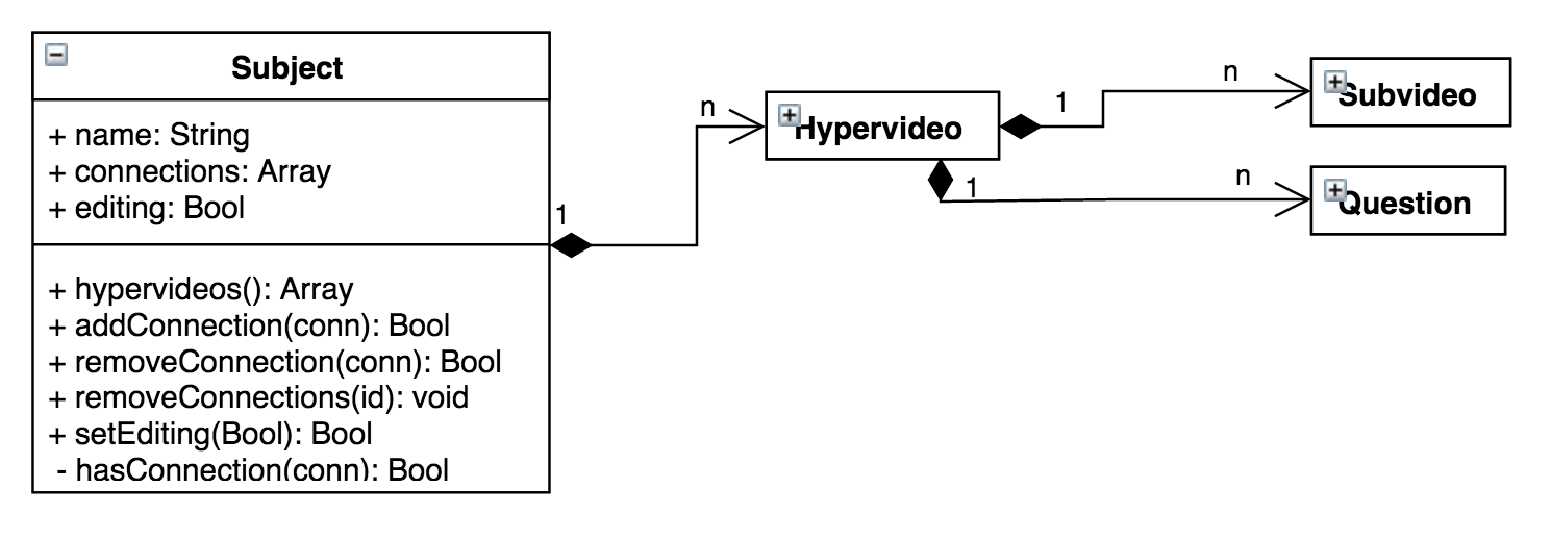
\includegraphics[width=.7\linewidth]{figuras/curso.eps}
  	\caption{Diagrama da estrutura do curso proposto}
  	\label{fig:curso}
\end{figure}

Para que fosse possível desenvolver uma adaptação da navegação que utilizasse a QRN, foi necessário modelar também a estrutura do curso que comportasse os hypervídeos e as informaçõs necessárias para os cálculos. Dessa forma, é proposto que um curso possua também, uma estrutura de grafo que tenha como vértices os seus Hypervideos, e que as conexões criadas pelo professor representem as ligações conceituais entre os tópicos apresentados em cada hypervídeo. A figura \ref{fig:curso} apresenta o modelo relativo ao curso que foi denominado \textit{Subject}.

A próxima modelagem feita foi referente aos dados do usuário: cursos que assiste, cursos construídos por ele, percentual de conclusão de um curso, questões respondidas, hypervideos assistidos, etc. Todas essas informações requereram modelos que vinculassem cada elemento de um curso ao usuário para que se pudesse calcular os coeficientes de quantização para os nodos da rede. A figura \ref{fig:userdata} mostra o modelo de domínio completo do \textit{software}.

\begin{figure}[h!]
	\centering
  	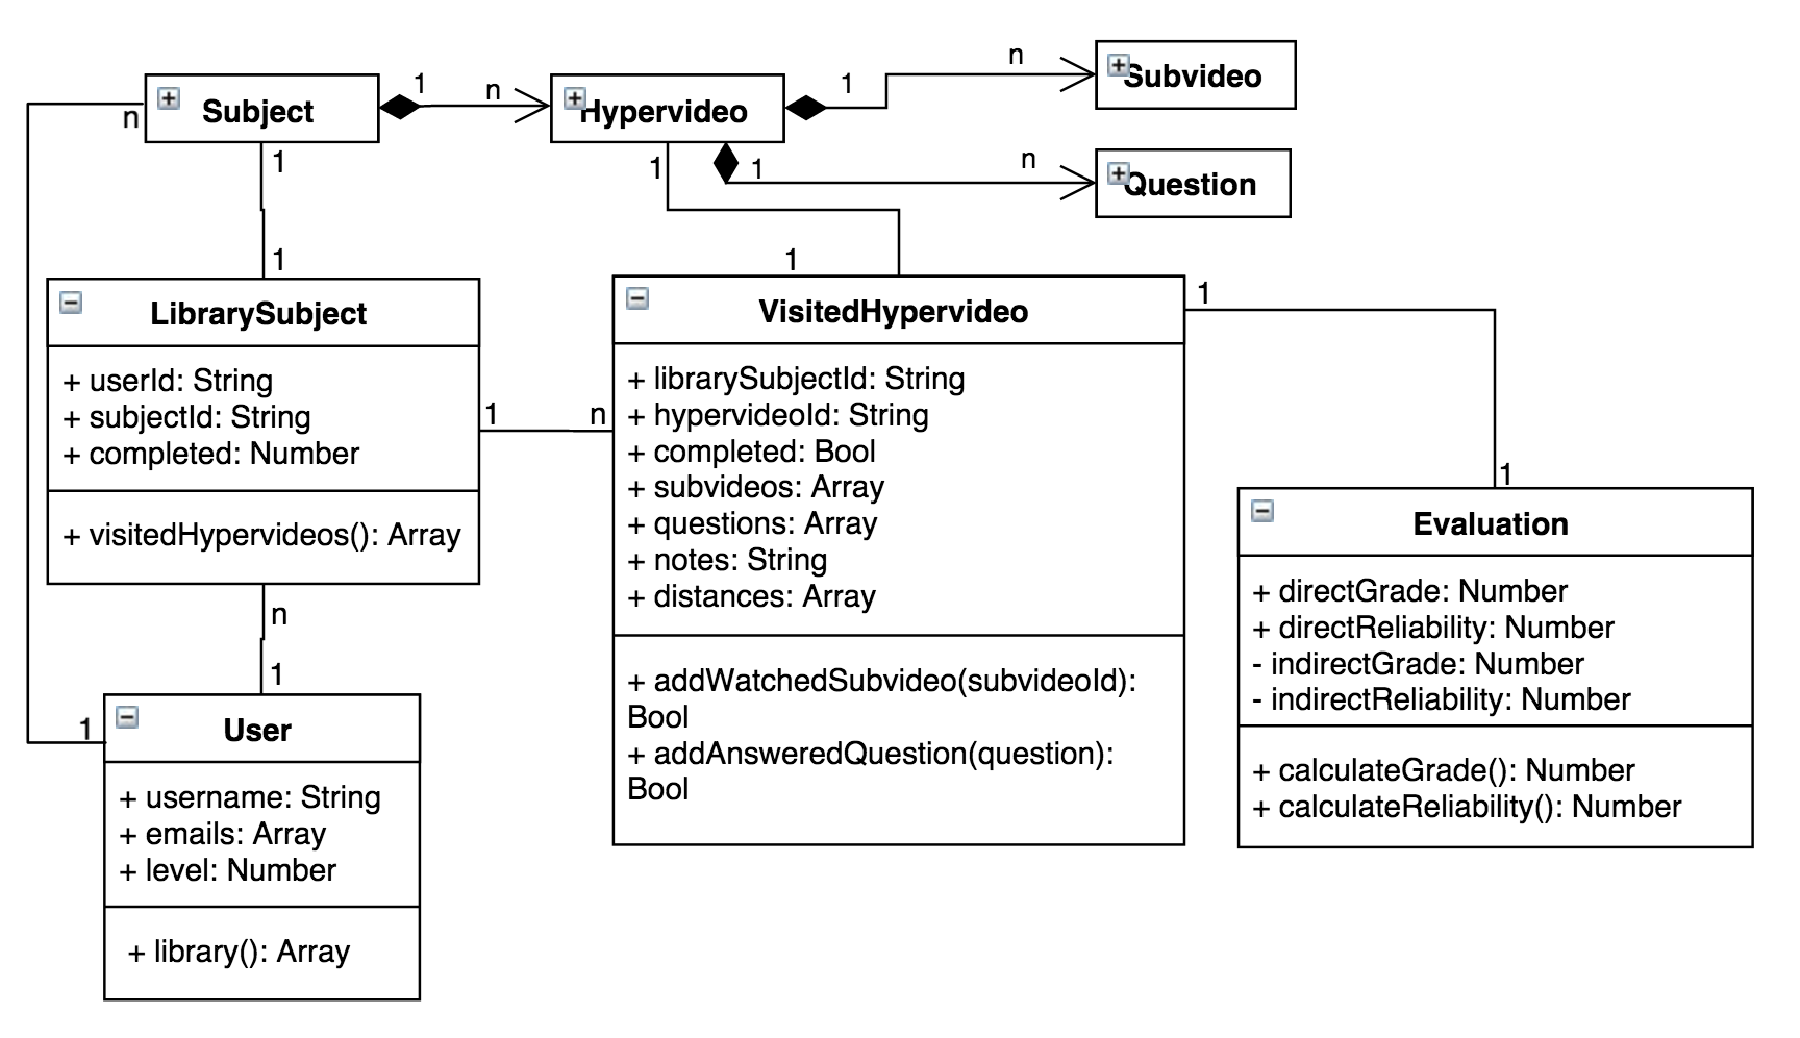
\includegraphics[width=.8\linewidth]{figuras/userdata.eps}
  	\caption{Diagrama sobre informações referentes a relação usuário \(\times\) curso}
  	\label{fig:userdata}
\end{figure}

Como a quantização da rede é definida de forma diferente para cada usuário, os cálculos da avaliação e confiabilidade diretas e indiretas devem estar vinculados ao objeto que interconecta o usuário ao nodo da rede que se pretende calcular a quantização. Dessa forma, para cada usuário que se cadastre na rede e assista a algum curso, uma quantização diferente será gerada segundo a sua interação com o sistema.

\section{Suporte Tecnológico}

Sobre o ponto de vista arquitetural, foram elicitadas ferramentas que proporcionassem maiores facilidades para o desenvolvimento do sistema. Nesse sentido, foram selecionados três \textit{frameworks} que possibilitam o desenvolvimento de aplicações \textit{web} com certo nível de abstração arquitetural, que são mantidos segundo licenças de software livre e que possuem comunidades ativas. Sendo estes: Grails \cite{grails2015}, Ruby on Rails \cite{rubyrails2015}, e Meteor \cite{meteor2015}. 
\\
\\

Para avaliar as ferramentas selecionadas, foi construído um cenário de prova de conceito, com a finalidade de verificar o esforço necessário para se implementar um pequeno software de manutensão de usuários nas três ferramentas. Os resultados coletados são descritos na tabela \ref{tab:tempo} abaixo:

\begin{table}[h!]
	\centering
	\begin{tabular}{| c | c |}
		\hline
		\textit{Framework} & Tempo \\
		\hline
		Meteor & 37 min \\
		\hline
		Rails & 44 min \\
		\hline
		Grails & 74 min \\
		\hline
	\end{tabular}
	\caption{Tempo para implementação da funcionalidade}
	\label{tab:tempo}
\end{table}

Os \textit{frameworks} Grails e Ruby on Rails possuem estilos arquiteturais bastante semelhantes, já que ambos são orientados a convensão, e possuem ferramentas de terminal interativo para criação e adição de elementos do sistema, como modelos, visões, controladoras e \textit{plugins}. Entretanto, o tempo para se desenvolver a funcionalidade com Ruby on Rails foi menor devido aos menores problemas com a configuração do ambiente de desenvolvimento e dependências do \textit{framework}.

Uma das vantagens da utilização do Ruby on Rails para o desenvolvimento é que a comunidade é bastante ativa e existe documentação abrangente sobre vários dos plugins que são disponibilizados para a plataforma. Porém, a configuração de uma ferramenta para renderização no cliente não é trivial e as complicações com a construção de APIs para comunicação remota e com a utilização de plugins JSON para recuperar dados do servidor impossibilitaram a construção da funcionalidade com este recurso.

Para a plataforma Grails, os mesmos problemas foram encontrados para a construção de uma aplicação com renderização no cliente, além dos problemas com configuração de ambiente e tempo de desenvolvimento da funcionalidade. A vantagem em se optar por utilizar uma ferramenta Java é a facilidade em se adicionar recursos multiagentes para tutoria inteligente, já que existem ferramentas consolidadas como o JADE \cite{jade2015} que são mantidas nessa linguagem. Como o foco deste trabalho não abrange o desenvolvimento de agentes, este \textit{framework} foi descartado.

O processo de instalação e utilização da plataforma Meteor foi o mais simples dentre as opções, todas as dependências do sistema são mantidas por meio do gerenciador de pacotes do Node.js \cite{nodejs2015} e foram instaladas sem nenhum empecilho. Apenas o processo simplificado de instalação não garante ao Meteor sua escolha como plataforma de desenvolvimento, além disso, o tempo para se implementar a funcionalidade proposta foi o menor, apresentou maior facilidade na construção de aplicações com renderização no cliente, possui comunidade ativa e releases frequentes de novas versões e mantém também mecanismos de teste e depuração para as aplicações, em sua maioria sob licenças de software livre compatíveis com GPL v3 adotada neste projeto.

A opção por uma ferramenta que facilite a renderização no cliente é uma necessidade da proposta para construção do curso, já que para criar um grafo de hypervideos em um curso, ou um grafo de subvideos e questões dentro de um hypervideo, tem-se a necessidade de se construir uma biblioteca para permitir a utilização do sistema sem que, a cada interação, se gere uma nova renderização da página proveniente do servidor, e que evite perda de dados caso ocorra falha de conexão com a \textit{internet}. Arquiteturas construídas com Ruby on Rails ou Grails não oferecem suporte esse tipo de interação, exigindo bibliotecas externas à plataforma e o conhecimento em linguagens de programação diferentes das utilizadas nativamente no \textit{framework}, como \textit{JavaScript} ou \textit{CoffeScript}.

Com esta análise, optou-se pela plataforma \textit{Meteor} devido às facilidades encontradas, pela necessidade de domínio em apenas uma linguagem: o \textit{JavaScript} e também pela possibilidade de se incluir bibliotecas para componentes visuas \textit{web}, como o Polymer \cite{polymer2015}. A lista completa de pacotes e ferramentas utilizadas se encontra no Apêndice A. 

\section{Arquitetura do Sistema}

Antes de compreender a arquitetura do sistema proposto, é preciso compreender como o \textit{framework} funciona e quais as possibilidades para expansão ou modificação da arquitetura proposta pela plataforma. Cada instância da aplicação no cliente registra serviços segundo padrão \textit{publish-subscribe} para coleções providas pelo servidor. Nativamente, o \textit{framework} dá suporte apenas para registros de \textit{publish-subscribe} para dados definidos em coleções no banco de dados.

\begin{figure}[h!]
	\centering
	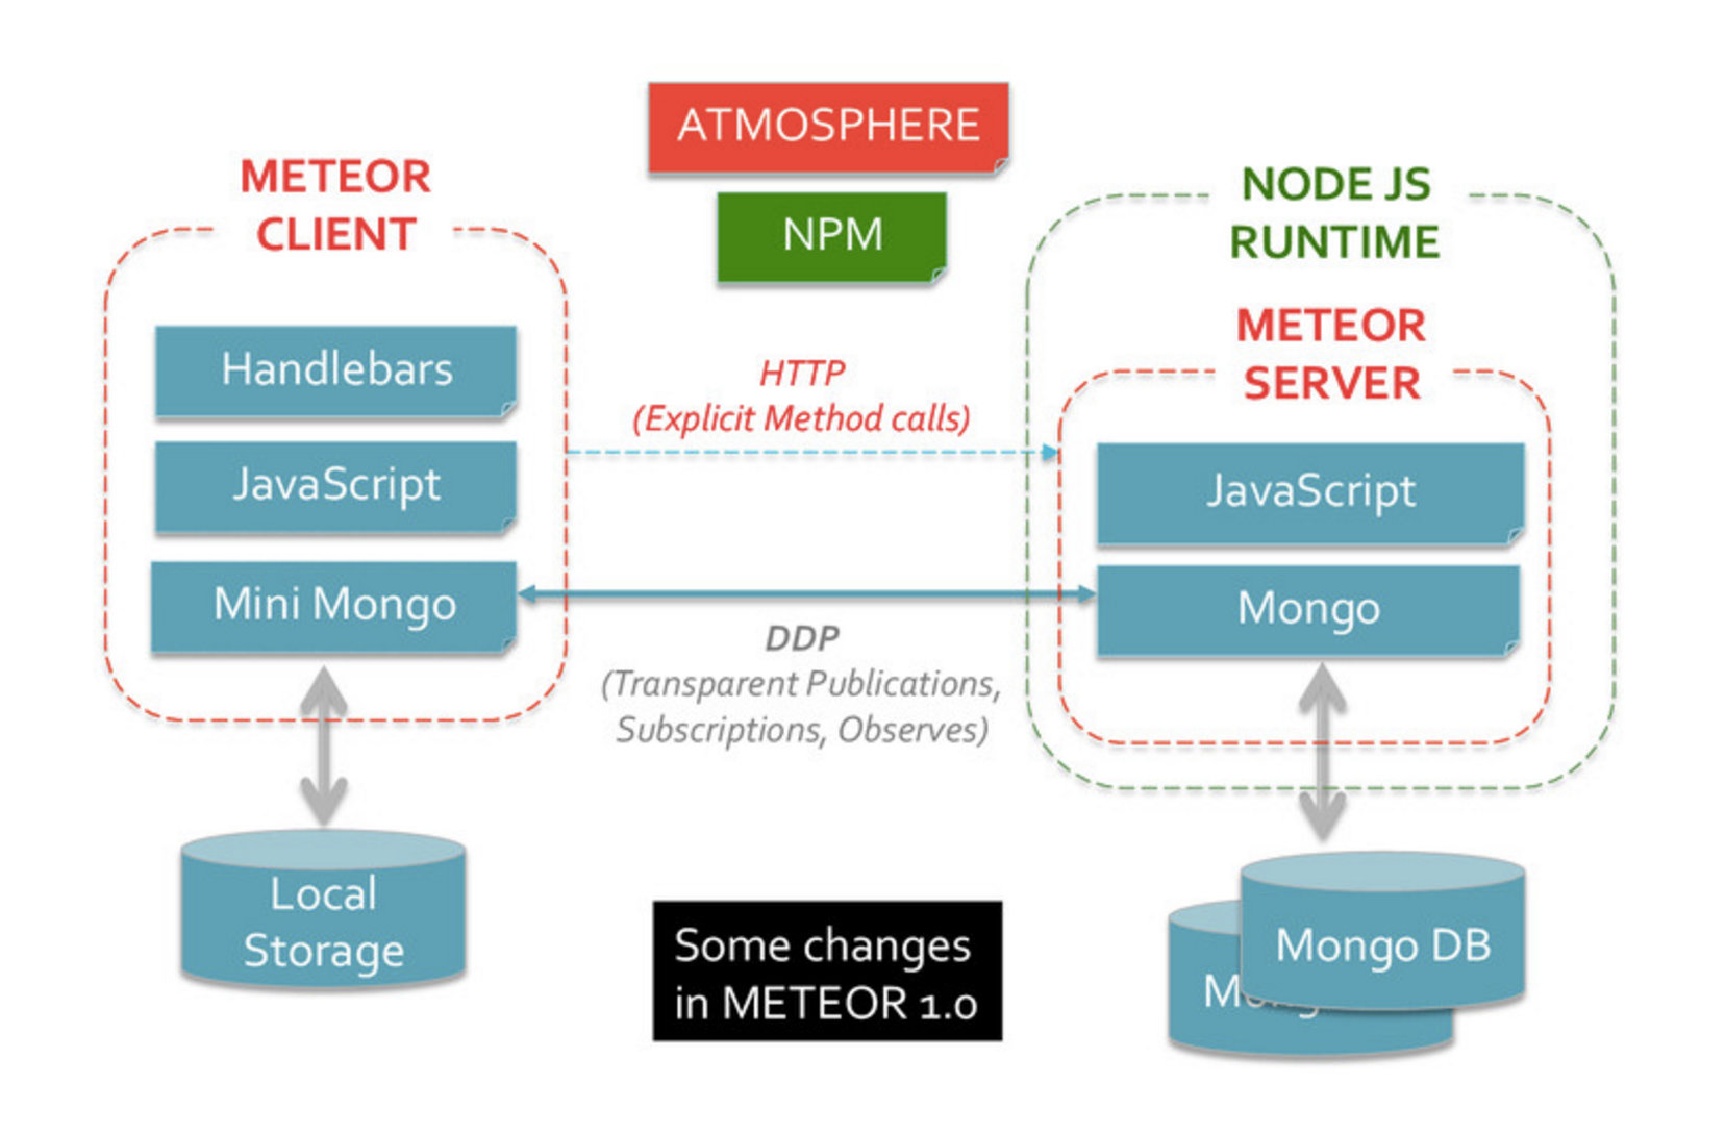
\includegraphics[width=.8\linewidth]{figuras/meteorarq.eps}	
  	\caption{Arquitetura Interna do \textit{Framework Meteor}}
	\small{Fonte: \cite{mongodb2015}}
  	\label{fig:meteorarq}
\end{figure}

O banco de dados utilizado pelo \textit{Meteor} é o MongoDB, que dá suporte a arquivos JSON, é facilmente escalável e possui boa performance. A aplicação no servidor roda em um \textit{container} Node.js e o \textit{framework} gerencia as trocas de dados cliente-servidor por meio de uma implementação em JavaScript da API do MongoDB que roda no navegador, chamada MiniMongo \cite{mongodb2015}. A figura \ref{fig:meteorarq} mostra como o \textit{Meteor}  gerencia os dados da aplicação e como são providos os serviços para os clientes. 

A plataforma não restringe, nem define um modelo arquitetural específico, abrindo espaço para que o desenvolvedor se encarregue de projetar de modo geral a arquietetura da aplicação. Inicialmente, uma aplicação possui arquitetura semelhante a mostrada na figura \ref{fig:subarq1} de forma que não existe separação nenhuma entre camadas lógicas, apenas entre servidor e cliente. A primeira forma da arquitetura proposta para o Sistema de vídeos Interativos incluiu à aplicação uma camada de modelo, separarando os dados do domínio, como ilustra a figura \ref{fig:subarq2}.

A lógica no cliente de uma aplicação \textit{Meteor} é gerenciada por uma biblioteca de renderização nativa (i.e. \textit{Blaze}), que responde reativamente às alterações que ocorrem nos dados locais, essa característica permite a criação de aplicações nativamente reativas e gera requisições menores por utilizar um protoco próprio e mais leve, denominado DDP (\textit{Distributed Data Protocol}) \cite{blaze2015}. 

\begin{figure}[h!]
	\centering
	\begin{subfigure}{.34\textwidth}
  		\centering
  		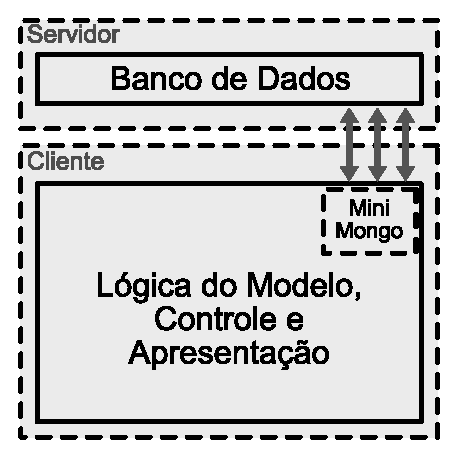
\includegraphics[width=.9\linewidth]{figuras/arquitetura1.eps}
  		\caption{estrutura inicial}
  		\label{fig:subarq1}
	\end{subfigure}%
 	 \begin{subfigure}{.34\textwidth}
  		\centering
  		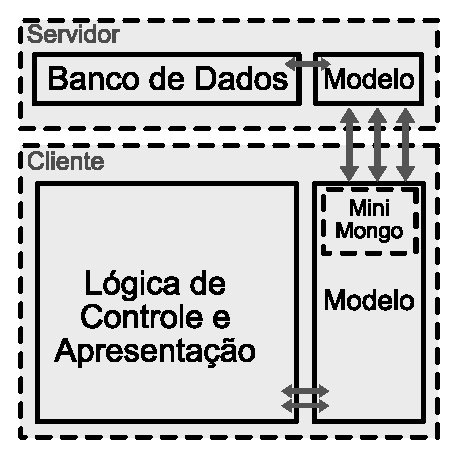
\includegraphics[width=.9\linewidth]{figuras/arquitetura2.eps}
  		\caption{modelo separado}
  		\label{fig:subarq2}
	\end{subfigure}%

	\begin{subfigure}{.34\textwidth}
  		\centering
  		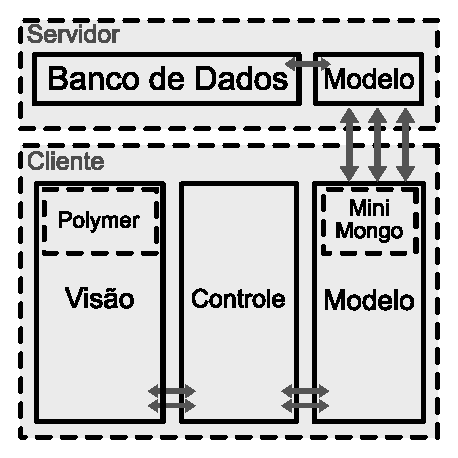
\includegraphics[width=.9\linewidth]{figuras/arquitetura3.eps}
  		\caption{visão separada}
  		\label{fig:subarq3}
	\end{subfigure}%
	\begin{subfigure}{.34\textwidth}
  		\centering
  		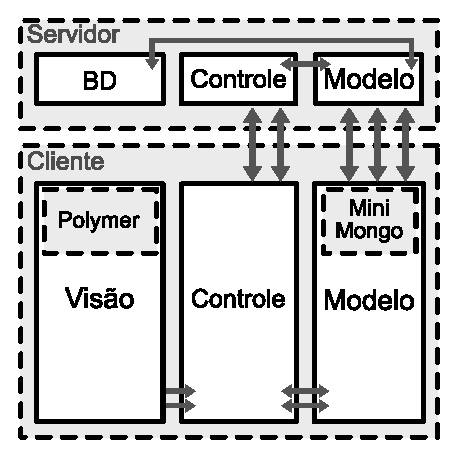
\includegraphics[width=.9\linewidth]{figuras/arquitetura4.eps}
  		\caption{controle organizado}
  		\label{fig:subarq4}
	\end{subfigure}
	\caption{Evolução da arquitetura da aplicação}
	\label{fig:arquitetura}
\end{figure}

Apesar das vantagens, o \textit{Blaze} possui alto acoplamento entre o controle e a visão, pois gerencia ambas as abstrações lógicas em um único arquivo, dificultando futuras manutenções da aplicação. Com a finalidade de se separar a lógica de controle e apresentação, foi adicionado ao sistema mais uma ferramenta, o \textit{Polymer} \cite{polymer2015}, que utiliza dados do modelo recebidos pelo \textit{Blaze} sempre que há alterações, e controla unicamente funções de apresentação, como posicionamento, cores, animações e outras operações da camada de visão. Esta versão é ilustrada pela figura \ref{fig:subarq3}.

Originalmente, aplicações \textit{Meteor} sincronizam os dados do cliente com o servidor automaticamente, sem que haja uma assinatura explícita dos dados (\textit{i.e. subscription}). Com o crescimento da base de dados do servidor, se torna inseguro e inviável que os dados sejam compartilhados entre todos os clientes ativos da aplicação. Para corrigir esta falha, a camada de controle foi extendida ao servidor com a função de limitar os dados que eram enviados para cada cliente por meio do padrão \textit{publish-subscribe}, sendo que apenas os dados necessários para a atual rota do usuário eram enviados para o cliente. Restrições de permissão para alteração dos dados foram criadas para manter a confiabilidade do banco. Esta é a versão atual da arquitetura, como ilustra a figura \ref{fig:subarq4}.

Agora que a arquitetura lógica foi descrita, deve-se verificar como esta foi implementada do ponto de vista de pacotes, com a finalidade de identificar a estrutura de diretórios e organização dos arquivos e dependências do projeto. O diagrama da fig. \ref{fig:arq_pacotes} apresenta a organização dos pacotes.

\begin{figure}[h!]
  	\centering
  	\includegraphics[width=.8\linewidth]{figuras/arq_pacotes.eps}
  	\caption{Diagrama de pacotes da arquitetura}
  	\label{fig:arq_pacotes}
\end{figure}

É possível perceber que no diagrama não existe nenhum pacote denominado controle, ou visão. Isto se deve ao fato de que o diretório em que se encontram os arquivos do \textit{Blaze} é geralmente denominado \textit{template}. No caso desta aplicação esse pacote é a camada de controle do cliente. A camada de visão se encontra no pacote \textit{public} juntamente com quaisquer outros recursos utilizados pela aplicação, como imagens.

Além disso, não existe nenhuma separação em pacotes no servidor, para modelo e controle. Até o momento deste trabalho, para as operações do controle no servidor são necessários apenas dois arquivos e para o modelo, apenas um, por esta razão, ainda não houve a necessidade de se criar pacotes diferentes.

O pacote de \textit{scripts} merece certo destaque pelo fato de gerenciar testes dos componentes visuais, rodar a aplicação em modo de \textit{profile} para análise de memória, consumo de CPU e tempo de resposta, e para gerar relatórios de cobertura e de análise estática de código, como aderência ao padrão de estilo de código \textit{JavaScript} para o \textit{Meteor}. Todas as saídas dos scripts são geradas no diretório oculto de \textit{output} e servem como base para parte do processo de integração contínua, melhor explicado no tópico seguinte sobre testes. 


\section{Testes}

O \textit{Velocity} é o \textit{framework} oficial de testes para aplicações \textit{Meteor}, suportando diferentes motores de teste como Mocha \cite{mocha2015}, Jasmine \cite{jasmine2015} ou Cucumber \cite{cucumber2015}, e permitindo que os resultados sejam exibidos em um componente reativo na interface da própria aplicação (fig. \ref{fig:teste_a}), ou via terminal (fig. \ref{fig:teste_b}), como um mecanismo para suporte em amibentes de integração contínua.

\begin{figure}[h!]
	\centering
	\begin{subfigure}{.5\textwidth}
  		\centering
  		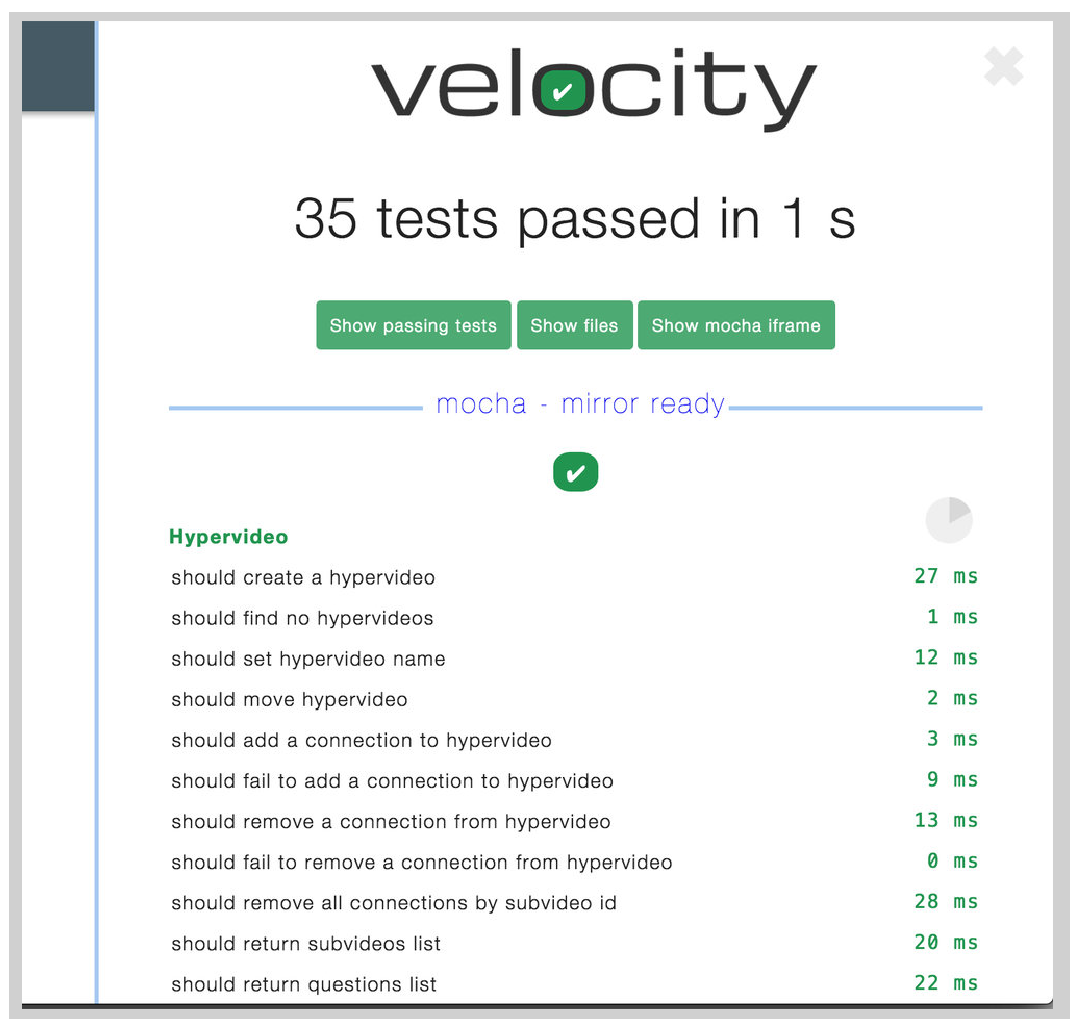
\includegraphics[width=.95\linewidth]{figuras/teste_a.eps}
  		\caption{componente \textit{Velocity} html}
  		\label{fig:teste_a}
	\end{subfigure}%
	\begin{subfigure}{.5\textwidth}
  		\centering
  		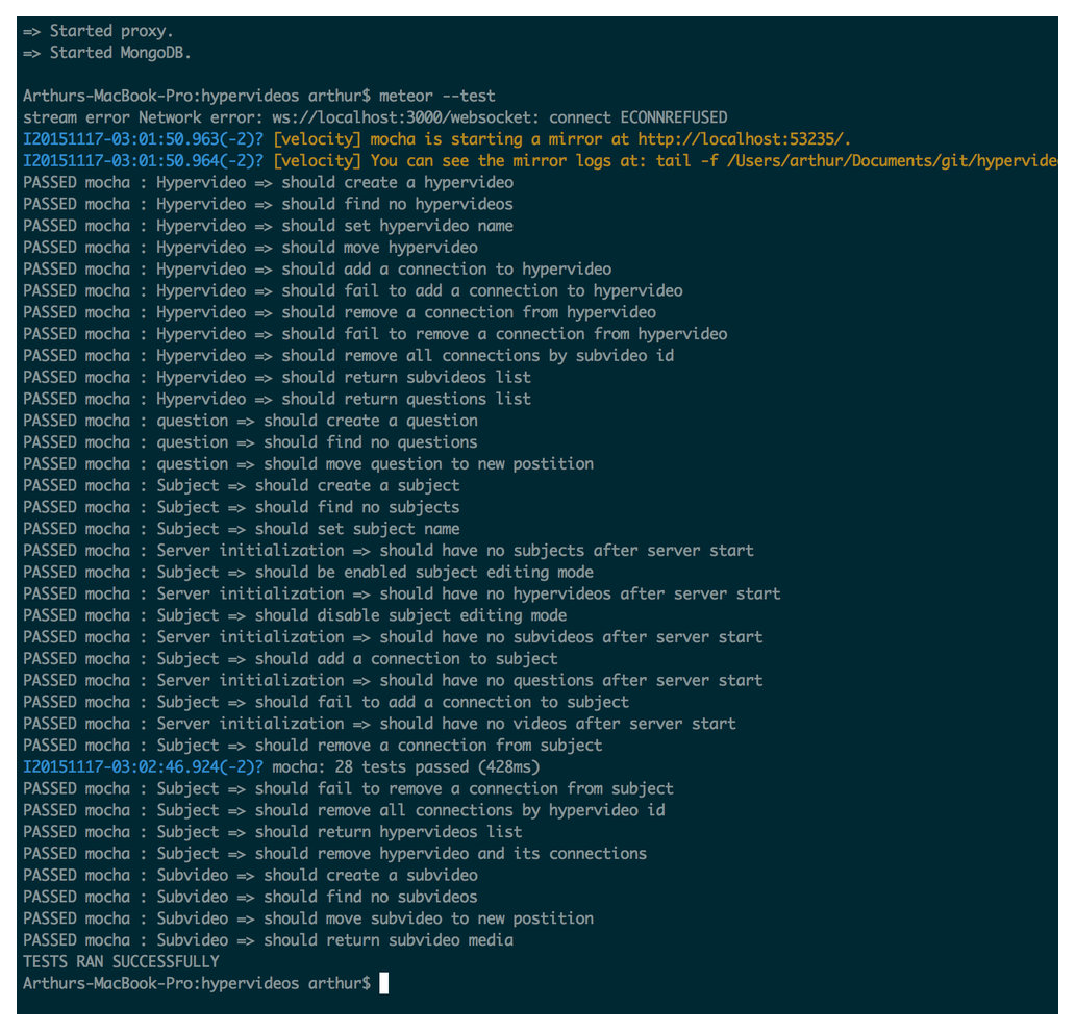
\includegraphics[width=.95\linewidth]{figuras/teste_b.eps}
  		\caption{\textit{Velocity} via terminal}
  		\label{fig:teste_b}
	\end{subfigure}
	\caption{Visualização dos resultados de teste da aplicação}
	\label{fig:testes}
\end{figure}

Para construção dos testes da aplicação foi utilizado o motor Mocha que fornece mecanismos para a construção de testes unitários e de integração que rodam com apenas um espelhamento da aplicação, reduzindo o consumo de memória, se comparado com o Jasmine que utiliza dois espelhos diferentes, um para testes unitários e outro para testes de integração \cite{jasmine2015}. Essa característica é importante para um ambiente de integração contínua pois reduz as configurações mínimas para a máquina que hospeda o serviço.

Além dos testes do \textit{Velocity} foi necessário configurar também um mecanismo de testes para os componentes construídos com o \textit{Polymer}. A comunidade que mantém o \textit{Polymer}, mantém também uma ferramenta de testes unitários e um \textit{plugin} para gerar relatórios de cobertura. O \textit{script} para os testes dos componentes é encontrado no diretório de \textit{scripts} e os relatórios de testes, como mostrado na figura \ref{fig:teste_polymer}, são gerados dentro da pasta de \textit{outputs}.

\begin{figure}[h!]
  	\centering
  	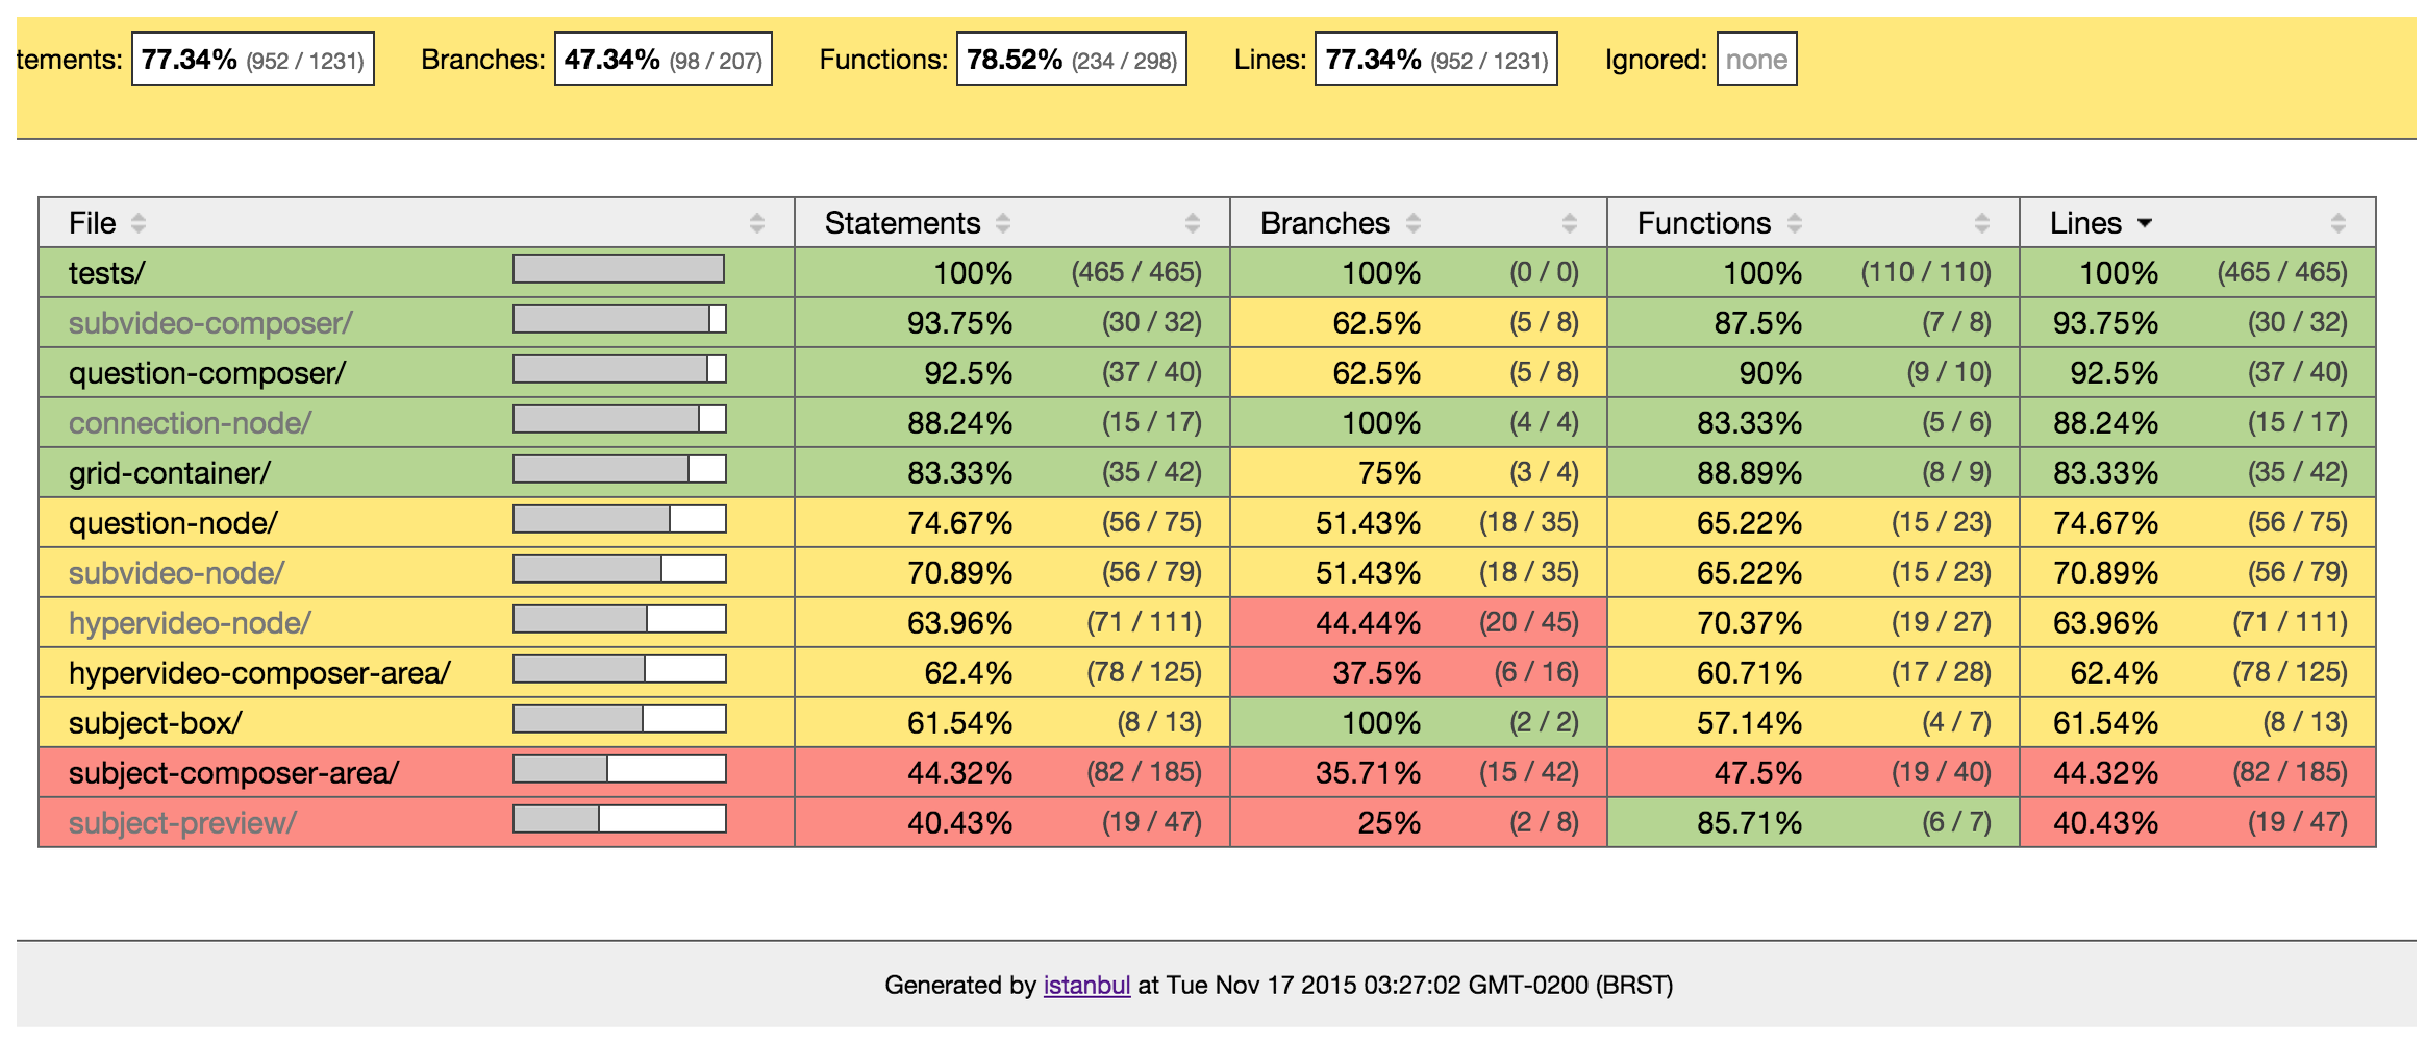
\includegraphics[width=.8\linewidth]{figuras/teste_polymer.eps}
  	\caption{Cobertura para componentes \textit{Polymer}}
  	\label{fig:teste_polymer}
\end{figure}

Após atualização para versão 1.2 do \textit{Meteor}, devido à refatorações na lógica de criação de aplicações espelhadas, não existem \textit{plugins} para gerar cobertura de código para a aplicação que seja compatível com o \textit{Velocity}, por essa razão, não são gerados relatórios de cobertura para a aplicação como um todo.

Além dos testes a nível unitário de integração utilizados, foi implementado um \textit{script} para configuração de uma ferramenta  para monitoramento de performance, como mostrado na figura \ref{fig:profile}. A ferramenta foi mais utilizada para analisar o tempo de resposta para as operações de \textit{publish} processadas no servidor, que não deve ultrapassar uma média de 300 ms \cite{kadira2015}.
\\ 
\\
\\
\\
\begin{figure}[h!]
  	\centering
  	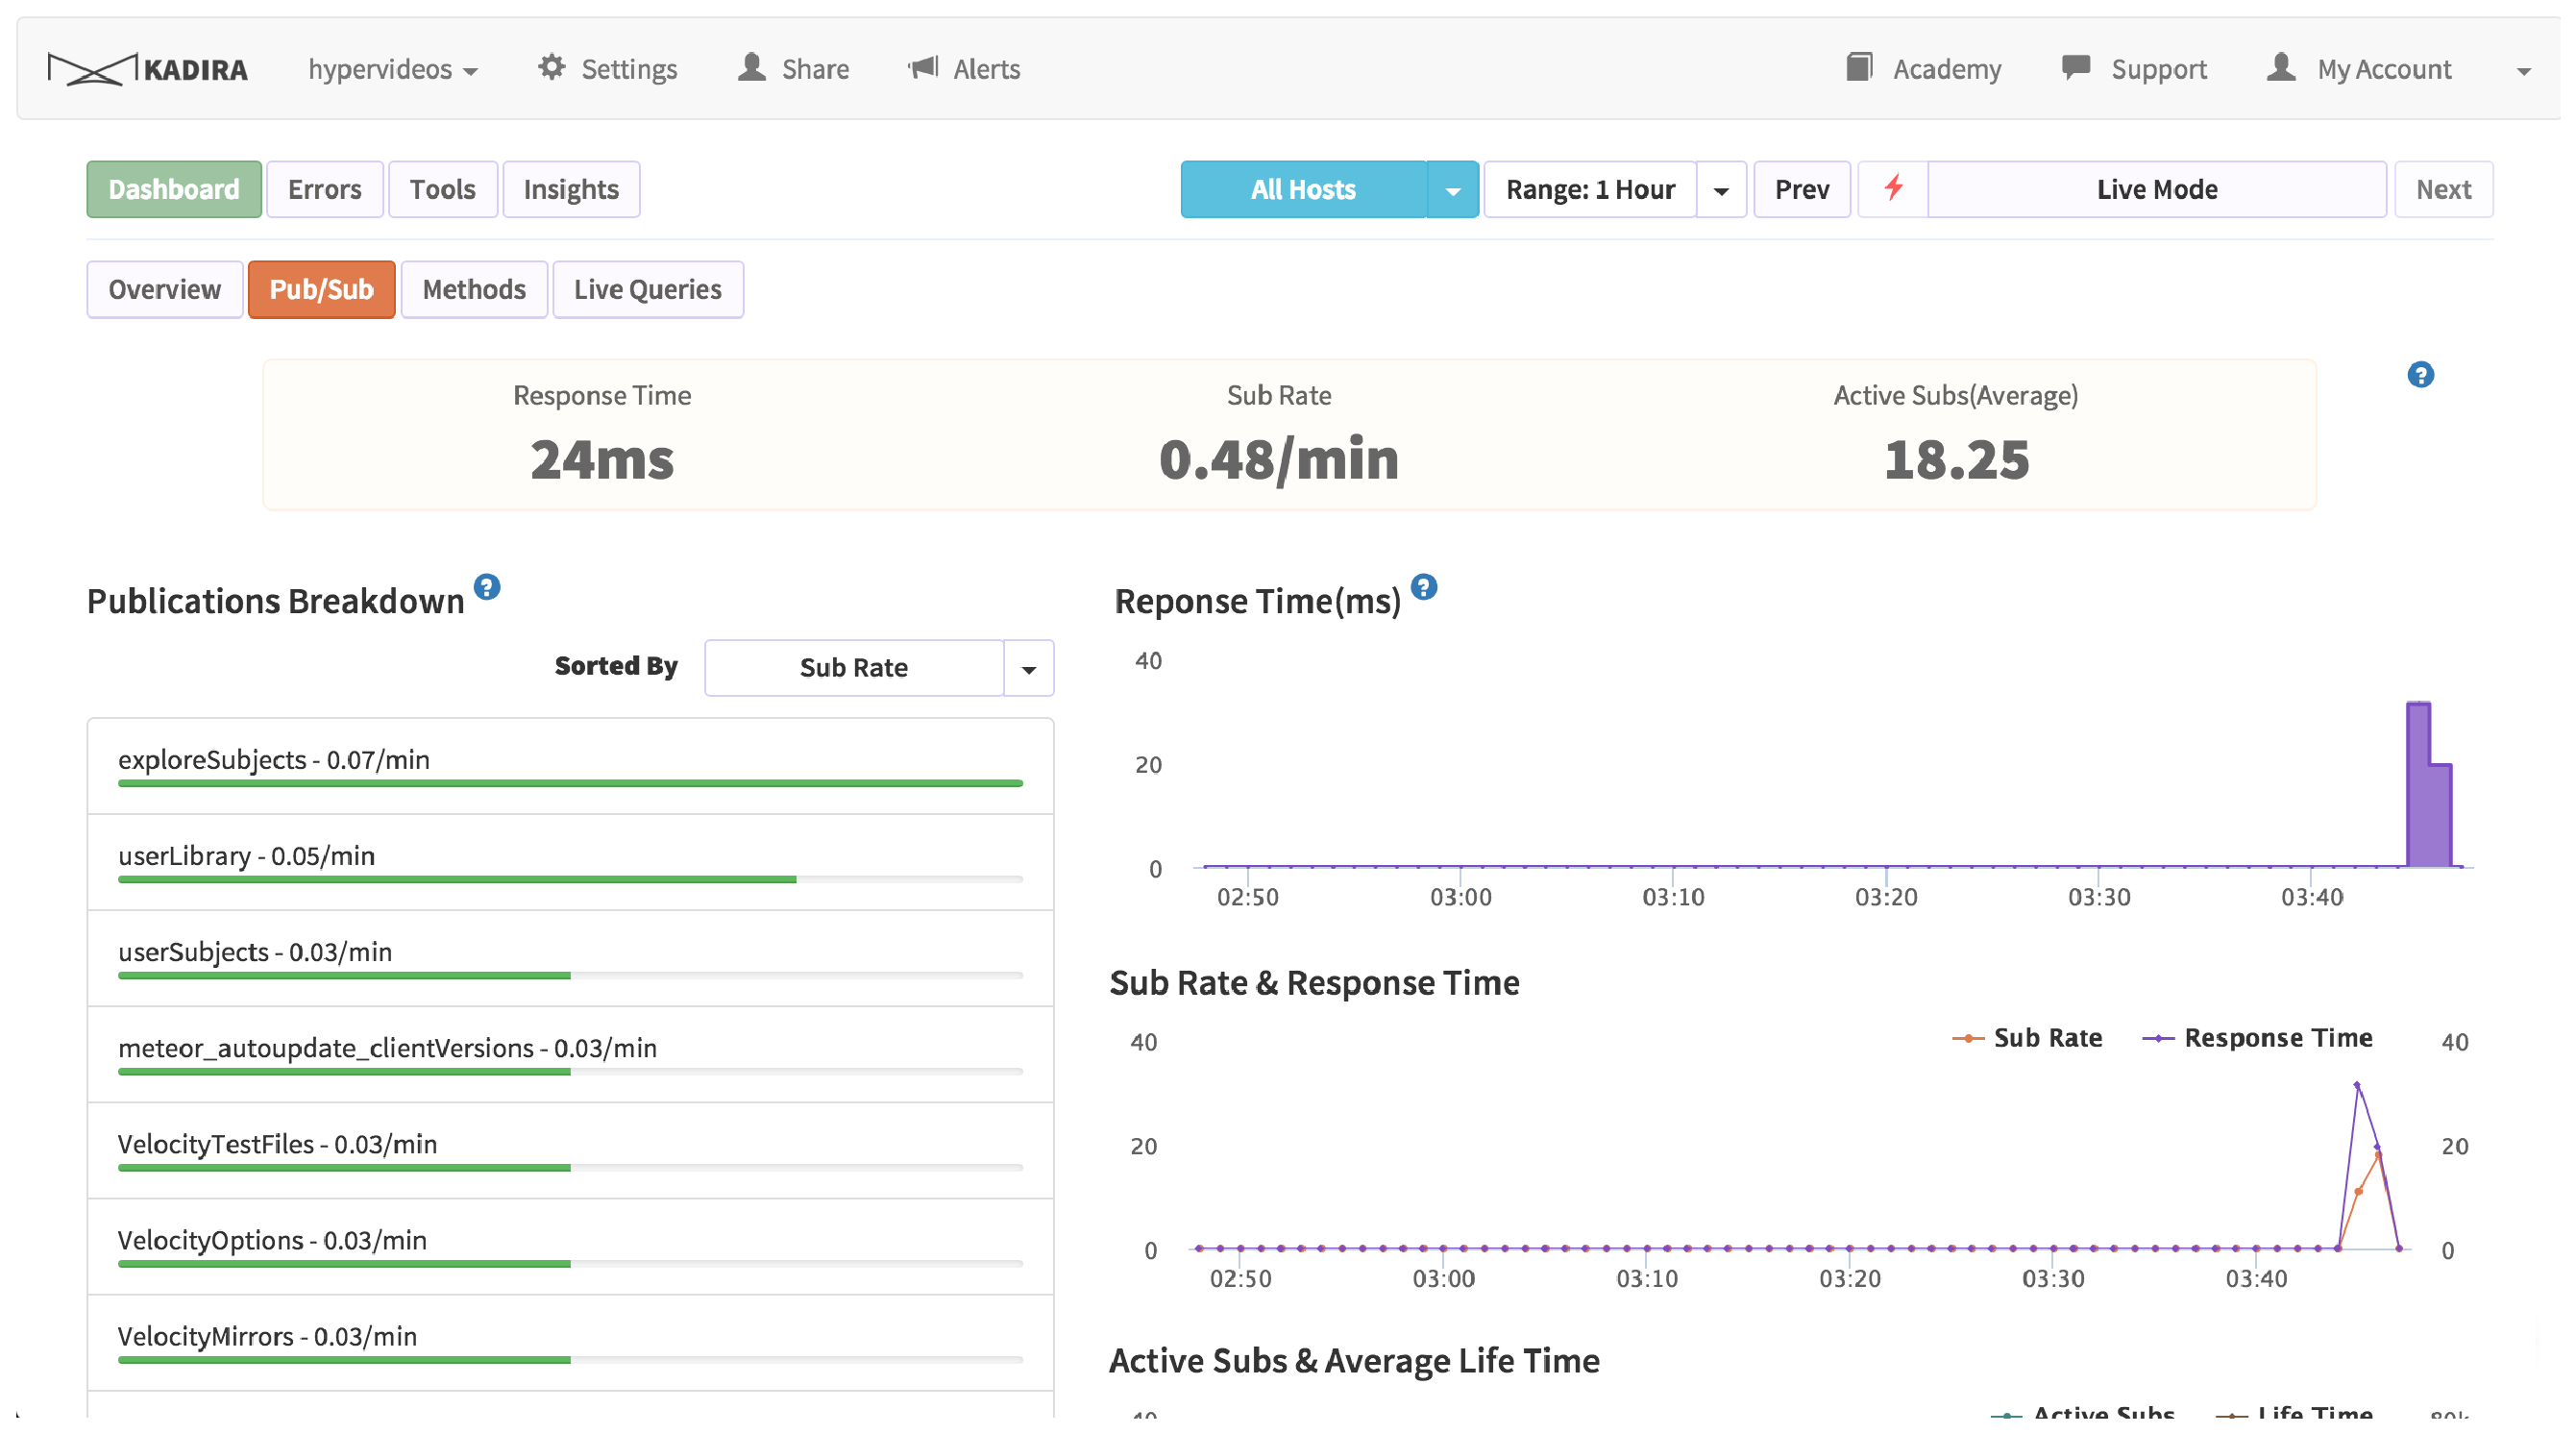
\includegraphics[width=.7\linewidth]{figuras/profile.eps}
  	\caption{Ferramenta para monitoramento de recursos utilizados pela aplicação}
  	\label{fig:profile}
\end{figure}

\section{Gerência de Configuração}